
\subsection{Methodology}

\subsubsection{Theoretical Formulation}

    \textbf{MLP Classifier} \\
    The MLP (Multilayer Perceptron) Classifier is chosen for our app due to its adaptability in handling diverse datasets, making it ideal for the variability in pet health profiles. Through iterative training, back-propagation, and refinement of internal weights, the MLP excels in recognizing nuanced symptom combinations indicative of specific diseases. This enhances diagnostic accuracy, a crucial aspect for caregivers with limited knowledge about canine health care, aligning perfectly without project's goal of providing a reliable pre-diagnosis system.
    
\begin{figure}[H]
\centering
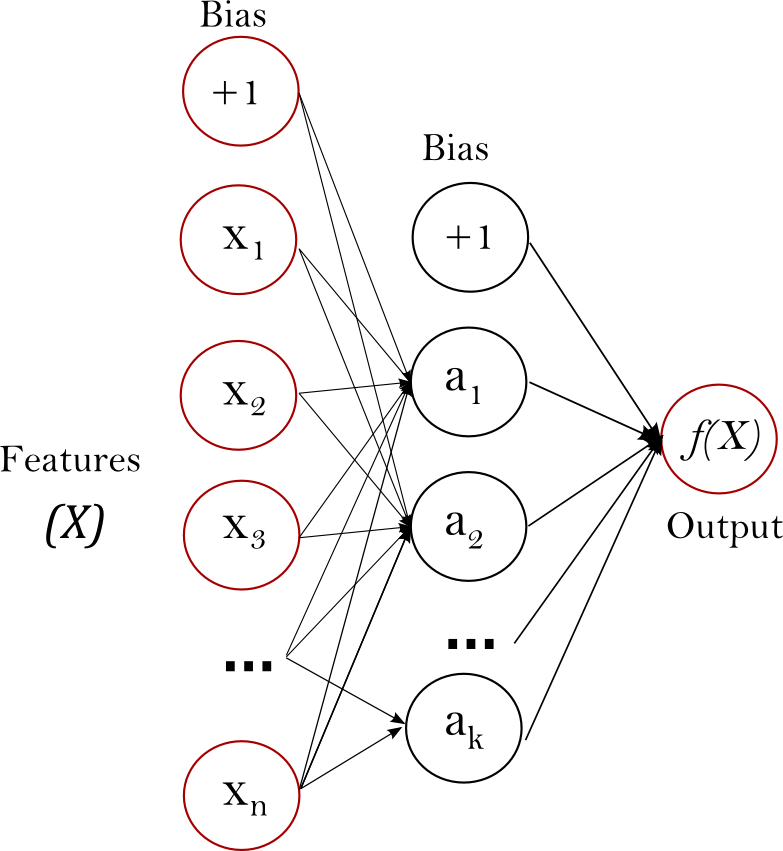
\includegraphics[width=0.53\linewidth]{img/MLP Classidier.png}
\\
 \caption{Training Loss Progression of MLP Classifier}
\label{fig:system-overview}
\end{figure}
\newpage
\noindent\textbf{{ResNet50}}\\
Deep learning, particularly neural networks, is chosen for its effectiveness in image classification tasks. In the context of HelloPet, accurate identification of pet breeds is essential for providing tailored advice and information. Deep learning algorithms excel in extracting complex features from images, making them ideal for breed identification.
The deep learning algorithm is specifically applied to the identification of pet breeds within HelloPet. Leveraging neural networks, it processes images and classifies the breeds, contributing to a comprehensive understanding of users' pets and enabling more personalized recommendations.
\begin{figure}[H]
\centering
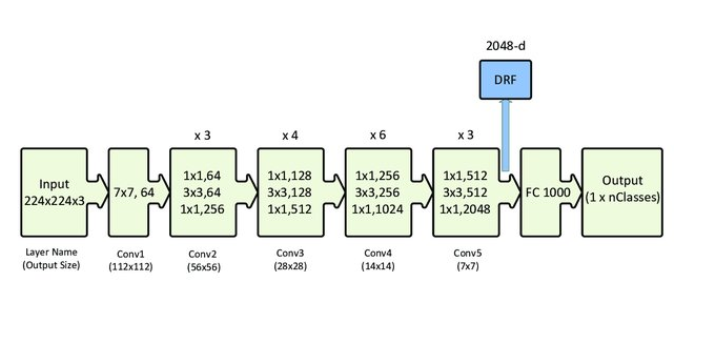
\includegraphics[width=0.75\linewidth]{img/lIAhY.png}
\\
\caption{ResNet50 diagram Source: \cite{22}}
\label{fig:system-overview}
\end{figure}

\noindent\textbf{Content Based Filtering}\\
Content based Filtering is a key component of HelloPet's recommendation system, strategically chosen to enhance the sense of community within the application. This content filtering technique relies on the attributes and characteristics of pet-related posts and products to generate personalized recommendations for pet owners. In the context of HelloPet, the system analyzes the features of individual pet-related posts and identifies similarities between them. This involves examining the characteristics, qualities, and interactions of pet-related activities and products to find commonalities. By leveraging this detailed understanding of pet-related content, HelloPet is able to offer users personalized suggestions and recommendations based on the features and qualities of items that align with their pet-raising preferences.   This method not only enhances user satisfaction by offering relevant and tailored recommendations but also creates a supportive environment where pet owners can explore new and exciting aspects of pet care based on the detailed attributes of pet-related content in the HelloPet platform.

    

